\documentclass[12pt]{article}
\usepackage{graphicx}
\usepackage{geometry}
\usepackage{listings}
\usepackage{xcolor}
\usepackage{float}
\usepackage{caption}

\geometry{a4paper, margin=1in}
\setlength{\parindent}{0pt}
\setlength{\parskip}{1em}

\definecolor{codegray}{rgb}{0.5,0.5,0.5}
\definecolor{backcolour}{rgb}{0.95,0.95,0.92}

\lstset{
    backgroundcolor=\color{backcolour},   
    basicstyle=\ttfamily\small,
    breakatwhitespace=false,         
    breaklines=true,                 
    captionpos=b,                    
    keepspaces=true,                 
    numbers=none,                    
    showspaces=false,                
    showstringspaces=false,
    showtabs=false,                  
    tabsize=2
}

\title{Big Data Analytics Group Assignment: Employee Data}
\author{Group Assignment}
\date{\today}

\begin{document}

\maketitle

\section*{Environment Setup}

The Hadoop environment was started using the \texttt{start-all.sh} command to bring up the HDFS NameNode, DataNode, and the YARN ResourceManager and NodeManager. The Java processes were verified using the \texttt{jps} command.

\begin{figure}[H]
    \centering
    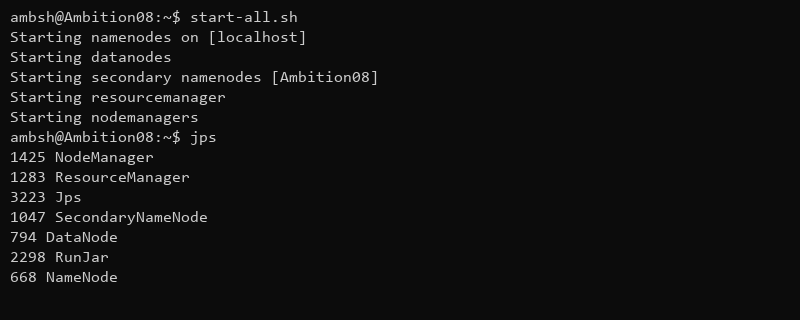
\includegraphics[width=\textwidth]{images/1_start_hadoop.png}
    \caption{Starting the Hadoop Environment and viewing JPS processes}
\end{figure}

Hive was initialized using the Beeline CLI in embedded mode connecting directly to the Derby Metastore. Environment variables were configured correctly before connecting.

\begin{figure}[H]
    \centering
    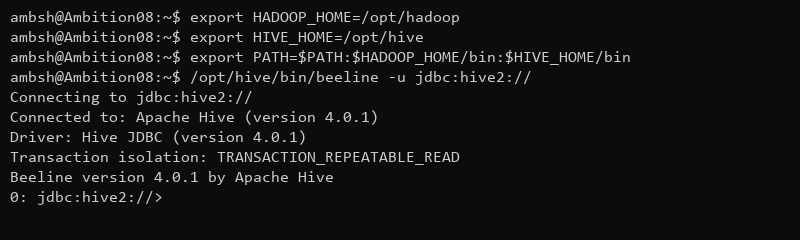
\includegraphics[width=\textwidth]{images/2_start_hive.png}
    \caption{Starting Hive using Embedded Beeline}
\end{figure}

\section*{1. Data Preprocessing}

The raw data was uploaded from the CSV file into a staging table (\texttt{EmployeeData\_Raw}). A cleaned table (\texttt{EmployeeData}) was then created to address data quality issues.
The following problems were addressed during this step:
\begin{itemize}
    \item \textbf{Missing Values:} \texttt{experience\_years} contained NULL values. Handled using \texttt{COALESCE(experience\_years, 0)}.
    \item \textbf{Inconsistent Casing:} \texttt{education\_level} had inconsistent casing. Fixed using \texttt{INITCAP()}.
    \item \textbf{Invalid Categorical Values:} \texttt{location} had entries listed as 'Remote' which is not a physical location. Fixed using \texttt{IF(location = 'Remote', 'Unknown', location)}.
    \item \textbf{Extreme Outliers:} \texttt{salary} had some monthly values instead of annual values (e.g. 50 instead of 50000). Handled using \texttt{IF(salary < 1000, salary * 1000, salary)}.
    \item \textbf{Whitespace Issues:} \texttt{date\_of\_marriage} had leading/trailing whitespaces. Handled using \texttt{TRIM()}.
\end{itemize}

\begin{figure}[H]
    \centering
    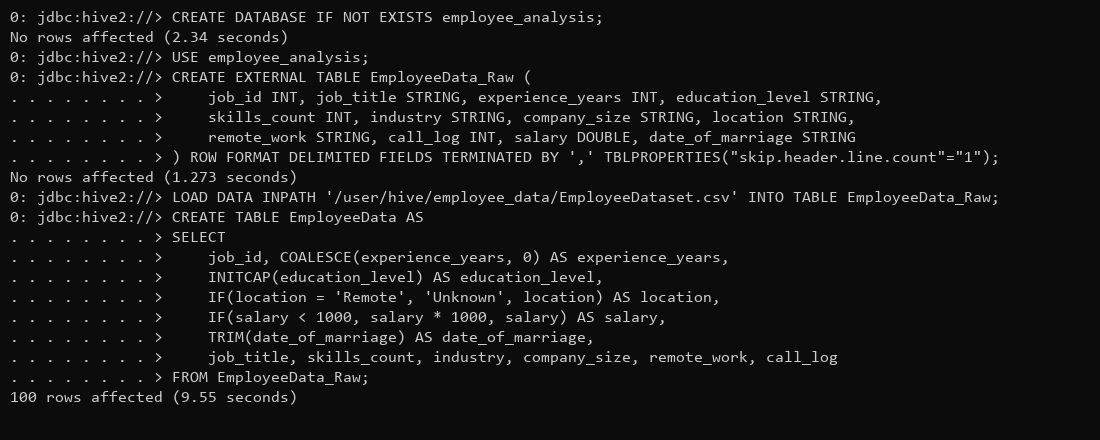
\includegraphics[width=\textwidth]{images/3_preprocessing.png}
    \caption{Data preprocessing and table creation}
\end{figure}

\section*{2. Split Job Title}

To cater for the first name and others, the \texttt{job\_title} column was split into two separate columns using Hive's \texttt{split()} and \texttt{substr()} functions.

\begin{figure}[H]
    \centering
    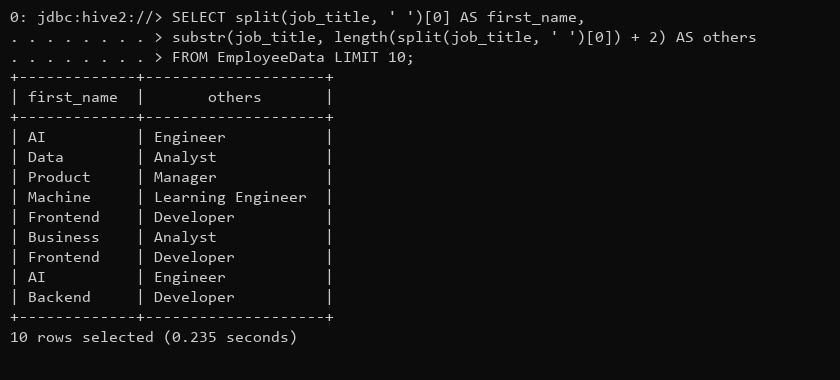
\includegraphics[width=\textwidth]{images/4_split_job_title.png}
    \caption{Output showing job title split into two columns}
\end{figure}

\section*{3. PhDs with Less Than 10 Years of Experience}

The query counted the number of employees with a PhD and less than 10 years of experience, grouped by their country.

\begin{figure}[H]
    \centering
    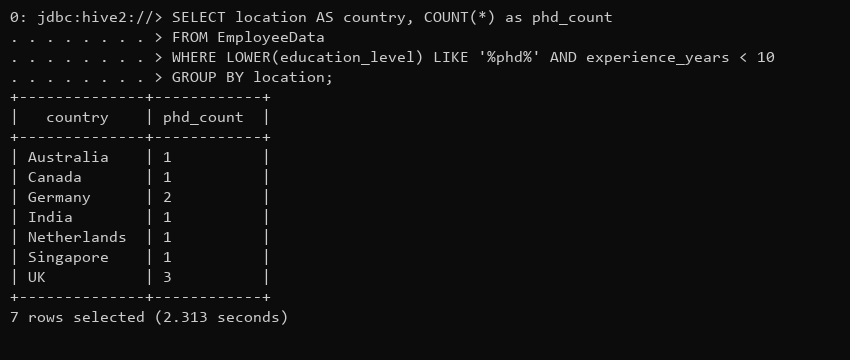
\includegraphics[width=\textwidth]{images/5_phd_count.png}
    \caption{Number of PhD employees with <10 years experience by country}
\end{figure}

\section*{4. Display Skills Count in Ascending Order}

The number of employees grouped by their \texttt{skills\_count} was calculated and displayed in ascending order.

\begin{figure}[H]
    \centering
    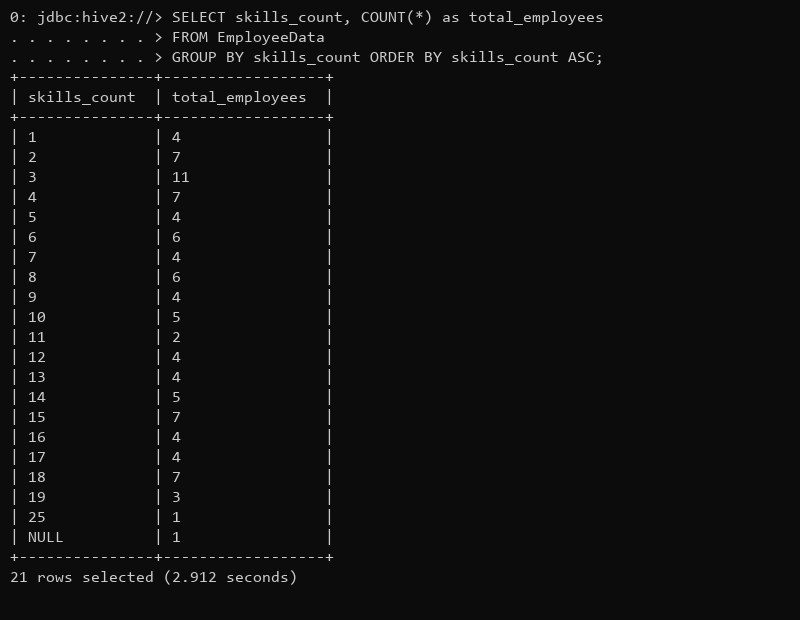
\includegraphics[width=\textwidth]{images/6_skills_count.png}
    \caption{Count of employees by their total skills in ascending order}
\end{figure}

\section*{5. Growth Rate (Call Log Totals and Averages)}

The growth rate representation included the total sum and average call log for PhD, Bachelor, and High School education levels.

\begin{figure}[H]
    \centering
    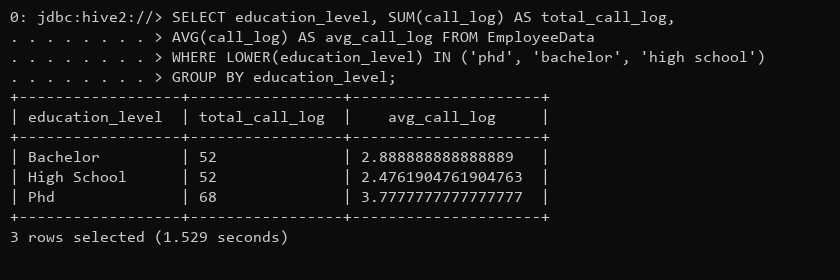
\includegraphics[width=\textwidth]{images/7_growth_rate.png}
    \caption{Total and average call log per education level}
\end{figure}

\section*{6. Predict Future Value for Call Log}

The predicted future value was calculated by assuming a 10\% growth (factor of 1.10) over the current average call log for the specified education levels.

\begin{figure}[H]
    \centering
    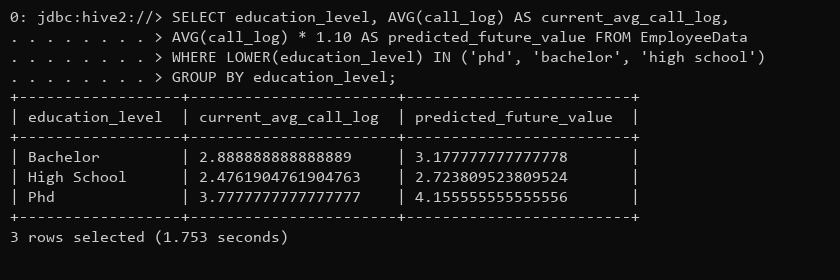
\includegraphics[width=\textwidth]{images/8_predict_future.png}
    \caption{Current average and predicted future call log values}
\end{figure}

\end{document}
